
\subsection{2.9. Точечные группы симметрии. Представление группы.} 

\par\bigskip

Для описания операций симметрии удобно использовать
специальный раздел математики - теорию групп.

\par\smallskip

Математическая группа - совокупность некоторых элементов
группы, связанных друг с другом определёнными правилами:

\par\smallskip

1) Любым двум элементам А и Б соответствует элемент тот же
группы В так, что А*Б=В.

\par\smallskip

2) Умножение ассоциативно

\par\smallskip

3) Существует единичный элемент Е, такой, что для любого
элемента группы Х:
 
 \par\smallskip
 
4) Если нет главных осей:

 \par\smallskip
 
Наряду с Х существует Y, также принадлежащей группе, что
Х*Y=Е (Y - элемент, обратный Х): $X\cdot E = E\cdot X = X$.

  \par\smallskip
  
Набор всех операций симметрии, оставляющих фигуру
неизменной, называется группой симметрии для данной фигуры.

\begin{figure}[H]
	\centering
	{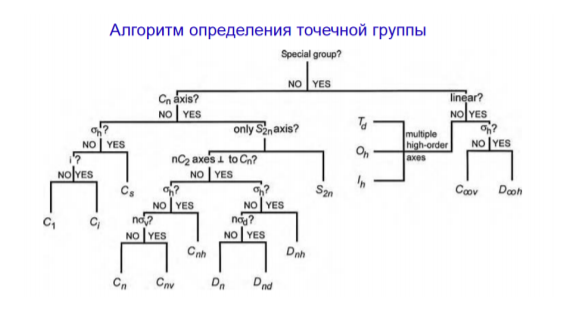
\includegraphics[scale=1.5]{29.png}}
\end{figure}


\begin{center}
	\textbf{Точечные группы симметрии:}
\end{center}

\begin{figure}[H]
	\centering
	{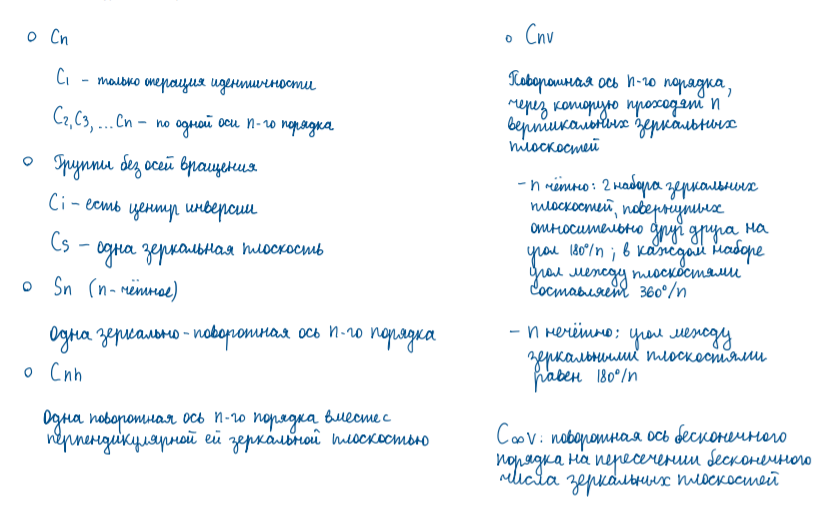
\includegraphics[scale=1]{54.png}}
\end{figure}

\begin{figure}[H]
	\centering
	{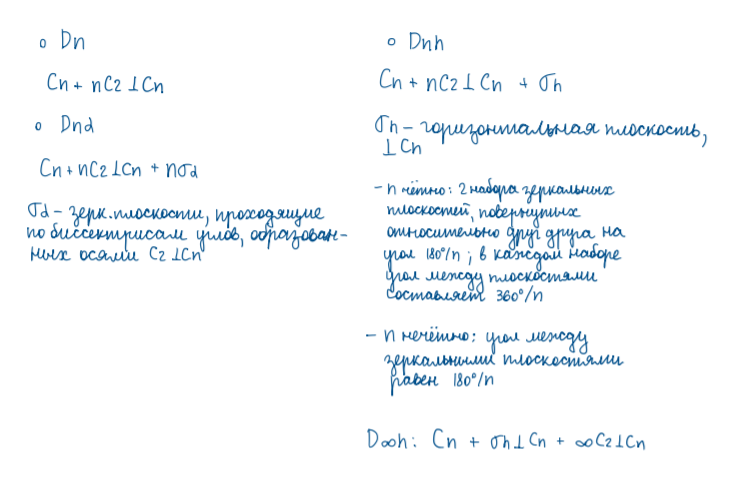
\includegraphics[scale=1]{55.png}}
\end{figure}

\begin{center}
	\textbf{Особые группы:}
\end{center}


\begin{figure}[H]
	\centering
	{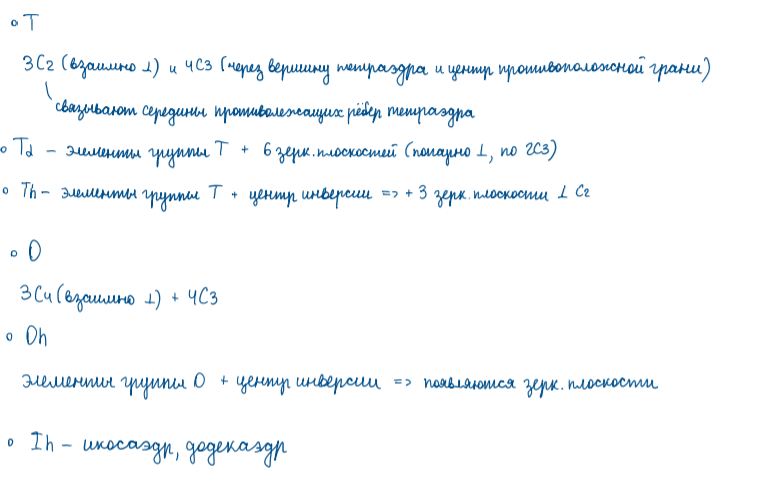
\includegraphics[scale=1]{56.png}}
\end{figure}

	Представление группы - это группа матриц, которые соответствуют
	действию каждой операции симметрии в данной точечной группе.
	Размерность матриц соответствует размерности рассматриваемого
	базиса из орбиталей или атомов.
	
	\par\smallskip
	
	
	Если умножить матрицу с исходным расположением орбиталей
	(атомов) слева на матрицу операции, получится матрица с
	расположением орбиталей (атомов), соответствующее таковому с
	учётом применённой операции симметрии. Умножение на
	единичную матрицу соответствует операции идентичности, оно
	коммутативно - не важно, слева или справа умножать матрицу.
	
	\begin{figure}[H]
		\centering
		{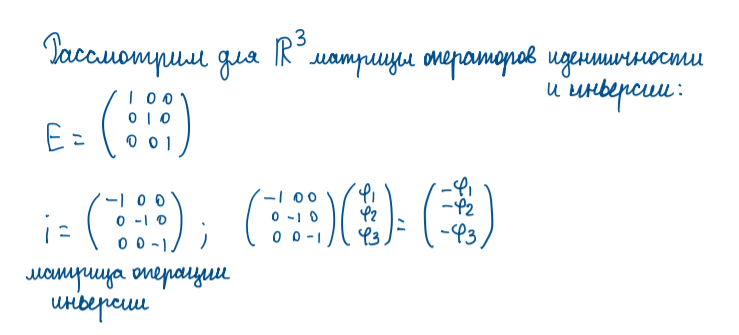
\includegraphics[scale=1]{30.png}}
	\end{figure}
	
	Для операций с поворотными осями важны матрицы поворота:
	
	\begin{figure}[H]
		\centering
		{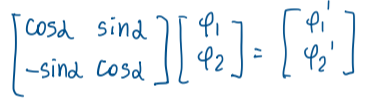
\includegraphics[scale=1]{31.png}}
	\end{figure}
	
	
	Для нахождения характеров матриц и формирования
	соответствующих неприводимых представлений используются
	базисы не из атомов, а из орбиталей.
	
	\par\smallskip
	
	Чтобы построить матрицу, нужно в строчку написать орбитали до
	применения операции, а в столбец - после. Рассмотрим на примере
	операции $С_2$ для молекулы воды:
	
		\begin{figure}[H]
		\centering
		{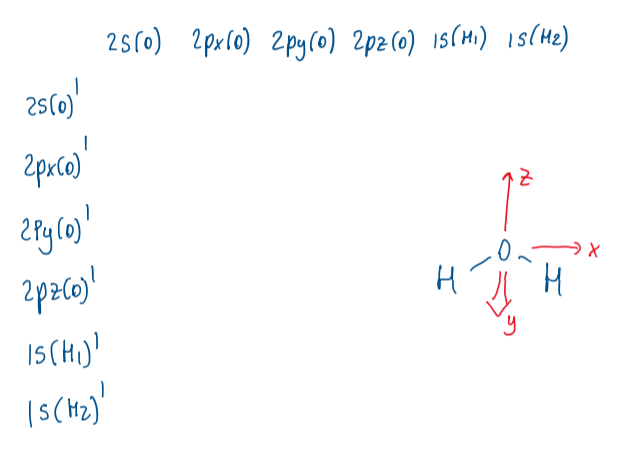
\includegraphics[scale=1]{32.png}}
	\end{figure}
	

	Если в результате применения операции орбиталь никак не
	изменилась, на пересечении для соответствующей орбитали надо
	поставить единицу. Если изменился знак волновой функции (для sорбиталей такого не будет), то будет -1. Если орбиталь изменила
	местоположение, на пересечении будет 0, а единица перейдёт на
	позицию, соответствующую другой орбитали, куда перешла
	исходная.
	
		\begin{figure}[H]
		\centering
		{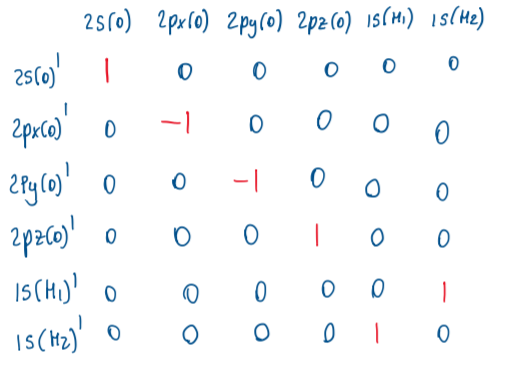
\includegraphics[scale=1]{33.png}}
	\end{figure}
	
		\begin{figure}[H]
		\centering
		{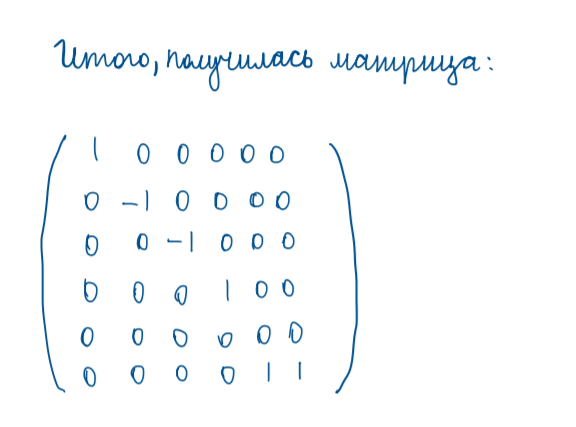
\includegraphics[scale=1]{34.png}}
	\end{figure}
	
	
	На самом деле, из всех этих чисел нам важны не все, но это скорее по
	теме следующего билета.
	
	\par\smallskip
	
	Чтобы задать представление группы, надо получить матрицы каждой
	операции в данной точечной группе.
	
	\par\bigskip
	\par\bigskip
	